\documentclass[letterpaper,11pt]{article}

\author{Jacob Thomas Errington (260636023)}
\title{Assignment \#3\\Honours advanced calculus -- MATH 248}
\date{8 November 2016}

\usepackage[margin=2.0cm]{geometry}
\usepackage{amsmath,amssymb,amsthm}
\usepackage{graphicx}

\newtheorem{prop}{Proposition}

\newcommand{\makebb}[1]{
  \expandafter\newcommand\csname #1\endcsname{\mathbb{#1}}
}
\newcommand{\parens}[1]{\left(#1\right)}
\newcommand{\D}{\mathrm{D}}
\renewcommand{\d}[2]{\frac{\mathrm{d}#1}{\mathrm{d}#2}}
\newcommand{\dd}[1]{\d{}{#1}}

\makebb{R}
\makebb{N}

\begin{document}

\maketitle

\section{Elliptical motion of the planets}

Consider the function $f : \R \to \R^2$ that defines the catesian coordinates
of a planet in terms of its angular position $\theta$ and the parameters
$a \geq b > 0$ of its elliptical motion.
\begin{equation*}
  f(\theta) = \parens{
    \begin{array}{l}
      a \cos \theta \\
      a \sin \theta
    \end{array}
  }
\end{equation*}

\emph{Kepler's equation} gives us the angular position in terms of the time $t$
elapsed since the planet passes through $(a, 0)$.
\begin{equation}
  kt = \theta -\epsilon \sin \theta
  \label{eq:kepler}
\end{equation}
where $\epsilon = \frac{c}{a}$ and $(c, 0)$ is the position of the Sun.

\begin{prop}
  It is possible to solve for $\theta$ in terms of $t$, for all $t \in \R$.
\end{prop}

\begin{proof}
  We will use the Implicit Function Theorem. First, we must put
  \eqref{eq:kepler} into a suitable form. Let $g : \R^2 \to \R$ be given by
  \begin{equation*}
    g(t, \theta) = kt + \epsilon \sin \theta - \theta
  \end{equation*}
  and consider $g(t, \theta) = 0$.
  Next, we verify $g(0, 0) = k \cdot 0 + \epsilon \sin 0 - 0 = 0$.
  We compute
  \begin{equation*}
    \partial_\theta g(t, \theta) = \epsilon \cos \theta - 1
  \end{equation*}
  Notice that this partial derivative is independent of $t$, and that it is
  nonzero whenever $\cos \theta \neq \frac{a}{c}$. Since $c > 0$ and $a > 0$,
  $\frac{a}{c} > 0$. Suppose $a < c$. Then we have a ``physical
  contradiction'', since the Sun will not be contained within the ellipse
  traced by the orbit of the planet. Hence $a \geq c$. We dispense with the
  case $a = c$ because the planet cannot pass through the Sun. Hence,
  physically, we deduce that $a > c$. Since $-1 \leq \cos \theta \leq 1$ for
  all $\theta$, there is no $\theta \in \R$ such that
  $\cos \theta = \frac{a}{c} > 1$. Therefore,
  $\partial_\theta g(t, \theta) \neq 0$ for all $t \in \R$.

  Next, since the partial derivatives of $g$ exist and are continuous, $\D g$
  exists, is equal to $J_g$, and is differentiable. Then by the Implicit
  Function Theorem, $\exists h : \R \to \R$ such that $\theta = h(t)$ for all
  $t \in \R$, i.e. we can write $\theta$ in terms of $t$.
\end{proof}

The implicit function theorem gives us an additional result concerning the
derivative of the implicit function, namely
\begin{equation*}
  \dd{t} h(t)
  = - \frac{\partial_t g(t, \theta)}{\partial_\theta g(t, \theta)}
  = \frac{k}{1 - \epsilon \cos \theta}
  = \frac{k}{1 - \epsilon \cos {h(t)}}
\end{equation*}

We are interested in the values of $g$ that produce extreme values of
$h^\prime$. These will coincide with the values of $\theta$ that produce
extreme values of $\cos \theta$, i.e. $0$ and $\pi$.

\begin{description}
  \item[Case] $\theta = 0$. Then $\cos \theta = 1$ and $1 > 1 - \epsilon > 0$,
    by the argument given in the above proof, so this gives us a maximum value
    for $h^\prime$. Physically, this makes sense since this is when the planet
    is closest to the Sun.

  \item[Case] $\theta = \pi$. Then $\cos \theta = -1$ and $1 + \epsilon > 1$.
    This gives us a minimum value for $h^\prime$. Again, this makes sense
    because this is when the planet is the farthest from the Sun.
\end{description}

We can't say exactly what the values of $t$ are that produce these maxima and
minima, because the Implicit Function Theorem is not constructive: it shows
that the implicit function exists without giving us its form.

\section{Lemniscate of Bernoulli}

Given the function $f : \R^2 \to \R$
\begin{equation}
    f(x, y) = (x^2 + y^2)^2 - 2(x^2 - y^2)
    \label{eq:lemniscate}
\end{equation}
consider $f(x, y) = C$ for constants $C$.

Expanding the definition of $f(x, y)$, we get
\begin{equation*}
    y^4 + y^2(2x^2 + 2) + (x^4 - 2x^2 - C) = 0
\end{equation*}
which is a quadratic equation in $y^2$. Solving for $y^2$ gives
\begin{align}
    y^2 &= -(x^2 + 1) \pm \sqrt{4x^2 + 1 + C} \notag \\
    y &= \pm \sqrt{-(x^2 + 1) \pm \sqrt{4x^2 + 1 + C}} \label{eq:lemniscate-y}
\end{align}

The curve in \eqref{eq:lemniscate} is symmetric along both the $x$ and $y$
axes since both coordinates are squared, so we can drop both $\pm$ in
\eqref{eq:lemniscate-y}. This gives us an equation for the top half of the
curve in \eqref{eq:lemniscate}. Using this formula we can sketch the level
curves, seen in figure \ref{fig:lemniscate-level-curves}.

\begin{figure}[ht]
    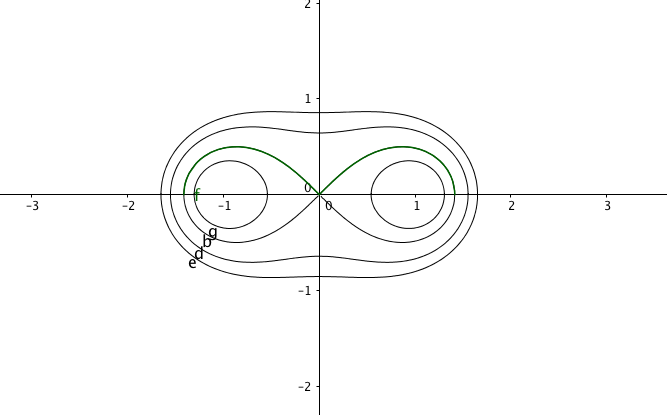
\includegraphics[width=\textwidth]{lemniscate-level-curves.png}
    \caption{
        Level curves of the function in \eqref{eq:lemniscate} for a few values
        of $C$.
    }
    \label{fig:lemniscate-level-curves}
\end{figure}

Next, let us investigate the partial derivates of $f$.
\begin{align*}
    \partial_x f(x, y) &= 2x(2x^2 + 2y^2 - 1)
    \partial_y f(x, y) &= 2y(2x^2 + 2x^2 + 1)
\end{align*}

In order to apply the Implicit Function Theorem, we need to verify a few
properties. Since the partial derivatives exist and are continuous,
$\D g$ exists and is equal to the Jacobian $J_g$. The second partial
derivatives also exist and are continuous, so $g$ is continuously
differentiable. We verify that $f(0, 0) = 0$.

Next, suppose $\partial_y f(0, 0) = 0$. Then either $2y = 0$ or
$2x^2 + 2y^2 + 1 = 0$. The latter case is a contradiction, since both $2x^2$
and $2y^2$ are nonnegative, so there is no choice for $x, y$ such that adding
the sum of (the double of) their squares to $1$ will give $0$. Hence, IFT can
be applied at all points $(x, y)$ where $y \neq 0$. By conferring with the
level curves, we can see that at least once, when $y = 0$, the curve crosses
the $x$-axis vertically, so the derivative with respect to $y$ becomes
infinite.

Finally, we wish to examine the points at which $y^\prime(x) = 0$.
The Implicit Function Theorem gives us an equation for $y^\prime$.
\begin{equation*}
    y^\prime(x) = \frac{\partial_x f}{\partial_y f}
    = \frac{2x(2x^2 + 2y^2 - 1}{2y(2x^2 + 2y^2 + 1}
\end{equation*}

Suppose $y^\prime(x) = 0$. Then, it suffices to consider
$2x(2x^2 + 2y^2 - 1) = 0$. So either $x = 0$ or $2x^2 + 2y^2 = 1$. Notice that
the latter case is the equation for a circle: the points on the curve
$f(x, y) = C$ determined by the latter case are precisely those where the
circle with radius $\frac{\sqrt{2}}{2}$

Substituting $x = 0$ into $f(x, y) = C$ gives $y^4 + y^2 - C = 0$. Solving for
$y^2$ gives
\begin{align*}
    y^2 &= \frac{-1 \pm \sqrt{1 + 4C}}{2} \\
    y &= \pm \sqrt{ \frac{-1 \pm \sqrt{1 + 4C}}{2} }
\end{align*}
So we can conclude that there is a corresponding $y$ coordinate when
$4C \geq -1$, and $\sqrt{1 + 4C} \geq 1$. These points where $x = 0$ and
$y^\prime(x) = 0$ do not lie in a circle with the other points where the
derivative is zero. This can be clearly seen in some of the level curves in
figure \ref{fig:lemniscate-level-curves}.

Substituting $y^2 = \frac{1 - 2x^2}{2}$ in $f(x, y) = C$ gives
\begin{equation*}
    x = \pm \frac{1}{2} \sqrt{\frac{5}{4} - C}
\end{equation*}
and substitu $x^2 = \frac{1 - 2y^2}{2}$ in $f(x, y) = C$ gives
\begin{equation*}
    y = \pm \frac{1}{2} \sqrt{C + \frac{3}{4}}
\end{equation*}
which gives us explicit points where $y^\prime(x) = 0$.

\end{document}
